\documentclass[12pt,a4paper]{article}

\usepackage[utf8]{inputenc}
\usepackage[T1]{fontenc}
\usepackage[brazil]{babel}
\usepackage{amsmath}
\usepackage{graphicx}
\usepackage{booktabs}

\usepackage[
    colorlinks=true,
    linkcolor=black,
    citecolor=black,
    urlcolor=black
]{hyperref}

\title{Análise dos dados de qualidade do ar}
\author{Annelise Poletto}
\date{7 de setembro de 2026}

\begin{document}

\maketitle

\section{Descrição dos dados}

Os dados utilizados neste relatório são provenientes do conjunto de dados
\textit{airquality}, disponibilizado na linguagem R \cite{RCore}. O conjunto
contém 153 observações referentes à qualidade do ar em Nova York.

A variável analisada neste relatório é \textit{Ozone}. Foram identificados
37 valores ausentes nessa variável. Dessa forma, as análises foram realizadas
considerando apenas as observações disponíveis para cada cálculo.

\section{Resultados}

A média da concentração de Ozone foi calculada para cada mês utilizando os
dados disponíveis. Conforme apresentado na Tabela \ref{tab:medias}, observa-se
uma variação da média de Ozone entre os meses analisados. O número de dias
medidos considera apenas as observações válidas, excluindo os valores ausentes.

\begin{table}[htbp]
\centering
\caption{Média de Ozone e número de dias medidos por mês}
\label{tab:medias}

\begin{tabular}{ccc}
\toprule
Mês & Média de Ozone & Dias medidos \\
\midrule
5 & 23.62 & 26 \\
6 & 29.44 & 9 \\
7 & 59.12 & 26 \\
8 & 59.96 & 26 \\
9 & 31.45 & 29 \\
\bottomrule
\end{tabular}

\end{table}

A Tabela \ref{tab:medias} mostra que as maiores médias de concentração de
Ozone ocorreram nos meses 7 e 8, com valores de 59.12 e 59.96,
respectivamente. Em contraste, os meses 5, 6 e 9 apresentaram médias menores.
Entretanto, o resultado do mês 6 deve ser interpretado com cautela, pois apenas
9 dias possuíam observações disponíveis.

A Figura \ref{fig:ozone} apresenta a distribuição dos valores de Ozone por mês,
incluindo boxplots e estimativas de densidade. A análise gráfica permite observar
diferenças tanto na concentração quanto na dispersão dos valores entre os meses.
Os meses 7 e 8 apresentam valores tipicamente mais elevados e maior variabilidade,
enquanto os meses 5 e 6 apresentam concentrações geralmente menores.

\begin{figure}[htbp]
\centering
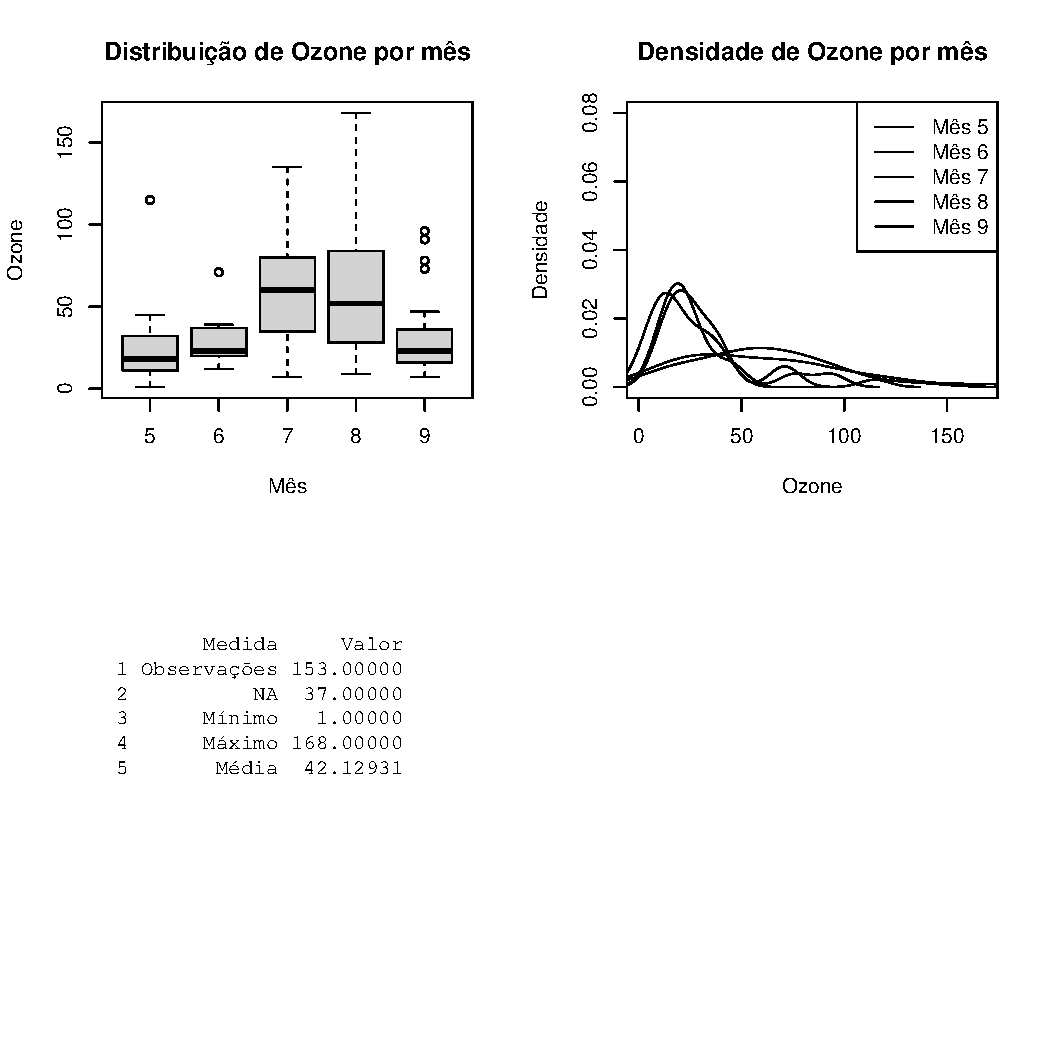
\includegraphics[width=0.85\textwidth]{figura.pdf}
\caption{Distribuição dos valores de Ozone por mês e resumo descritivo da variável}
\label{fig:ozone}
\end{figure}

A média utilizada nos resultados pode ser representada pela Equação
\eqref{eq:media}:

\begin{equation}
\bar{x} =
\frac{\sum_{i=1}^{n_{\text{válidos}}} x_i}
{n_{\text{válidos}}}
\label{eq:media}
\end{equation}

O denominador da Equação \eqref{eq:media} considera apenas os valores
disponíveis, excluindo as observações ausentes. Essa escolha é importante neste
conjunto de dados, pois a variável Ozone possui 37 valores faltantes.

De forma geral, os resultados indicam uma variação considerável da concentração
de Ozone ao longo dos meses analisados. Além da diferença entre as médias, a
Figura \ref{fig:ozone} evidencia mudanças na dispersão e no formato das
distribuições. A presença de valores ausentes também reforça a importância de
considerar o número efetivo de observações em cada mês ao interpretar os
resultados. A análise foi realizada utilizando recursos estatísticos da linguagem
R \cite{RCore,Venables}.

\bibliographystyle{plain}
\bibliography{referencias}

\section*{Declaração de uso de IA}

Foi utilizada uma ferramenta de inteligência artificial como apoio na estruturação
do código em LaTeX e na compreensão dos comandos utilizados. O conteúdo gerado
foi revisado e os resultados foram conferidos por meio da compilação do documento
e da comparação com os arquivos produzidos durante a análise.

\end{document}